\newpage
\begin{center}
    \Huge{\textbf{\underline{Exercise 4}}}
\end{center}

\vspace{0.45cm}

\begin{center}
    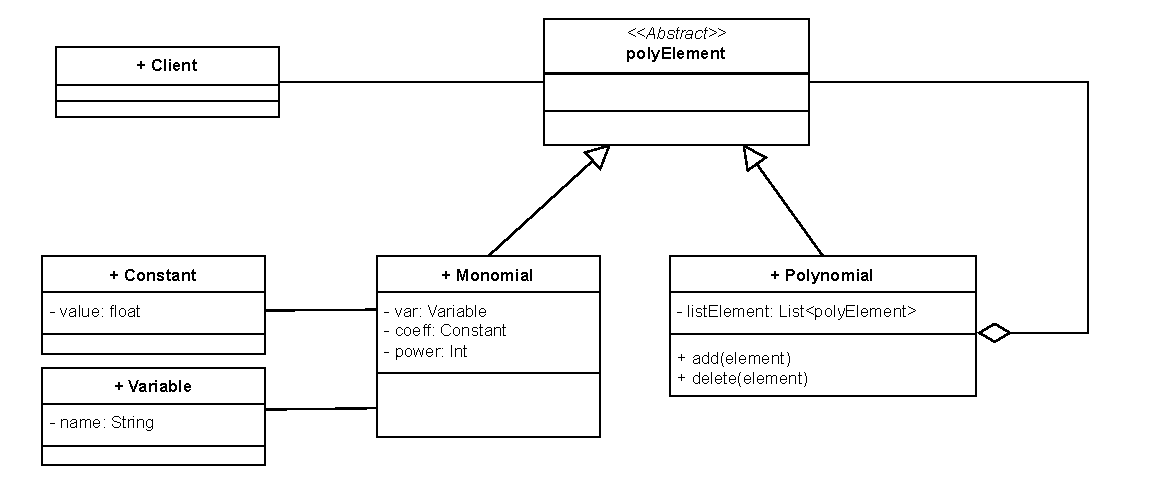
\includegraphics[height=0.22\textheight]{Exercices/EX4/ex4.drawio.pdf}
\end{center}

\vspace{0.25cm}

\begin{prettyBox}{Explication}{myblue}
We used the \texttt{Constant} and \texttt{Variable} classes to create the 
\texttt{Monomial} class, which holds the name of the variable, the power, and the coefficient. 
The \texttt{Monomial} is a leaf element, and the \texttt{Polynomial} is the complex element 
that holds a list of \texttt{Monomial}.
\end{prettyBox}

